\documentclass[11pt,a4paper]{article}
\usepackage[T1]{fontenc}
\usepackage[utf8]{inputenc}
\usepackage[margin=2.1cm]{geometry}
\usepackage{amsmath,amssymb,bm}
\usepackage{booktabs}
\usepackage{multirow}
\sloppy
\usepackage{graphicx}
\usepackage{float}
\usepackage{caption}
\usepackage{xcolor}
\usepackage[hidelinks]{hyperref}
\newcommand{\best}[1]{\textbf{#1}}
\newcommand{\warn}[1]{\textcolor{red!70!black}{#1}}

\title{A topological descriptor for magnetic textures\\
       \large What it measures, how it is computed, and why the scalar observables need it}
\author{}
\date{\today}

\begin{document}
\maketitle

\begin{abstract}
The three physical observables used so far --- magnetisation, nearest-neighbour spin
correlation and peak wavevector --- are all averages over the nanodot disk. A perturbation
of about $1\%$ of the image range, placed near the Nyquist frequency, moves each of them
slightly while changing an encoder's reading of a Hamiltonian parameter from $r=0.001$ to
$r=0.985$. This note introduces five descriptors of the topology of the $s_z$ level sets.
They are \emph{discrete}, so that perturbation cannot move them at all. On their own they
classify the six magnetic phases with a balanced accuracy of $0.831$, slightly above the
$0.813$ of the three scalars, and the two families together reach $0.888$ --- they are
complementary, not redundant.
\end{abstract}

\section{What is measured}

Let $s_z(\mathbf{r})$ be the projection stored in the dataset, restricted to the nanodot
disk $\mathcal{M}$ of radius $R_d = 18.25$ MUC. Fix a threshold $\tau$ and define two sets:
\[
  \mathcal{P} = \{\mathbf{r}\in\mathcal{M} : s_z(\mathbf{r}) > +\tau\},
  \qquad
  \mathcal{N} = \{\mathbf{r}\in\mathcal{M} : s_z(\mathbf{r}) < -\tau\}.
\]
Five numbers are extracted:

\begin{center}\small
\begin{tabular}{lll}
\toprule
Symbol & Name & Meaning \\
\midrule
$n_+$, $n_-$ & \texttt{n\_pos}, \texttt{n\_neg} & connected components of $\mathcal{P}$ and $\mathcal{N}$ \\
$\chi$ & \texttt{euler\_pos} & Euler characteristic of $\mathcal{P}$: components $-$ holes \\
$w$ & \texttt{wall\_frac} & fraction of in-disk neighbour pairs with $s_z(i)\,s_z(j)<0$ \\
$a_{\max}$ & \texttt{largest\_frac} & area of the largest component of $\mathcal{P}$, over $|\mathcal{M}|$ \\
\bottomrule
\end{tabular}
\end{center}

\section{Fundamento}

\paragraph{Why topology and not another average.}
The Euler characteristic is a \emph{topological invariant}: it is unchanged by any
continuous deformation of the set and moves only when a component appears, merges, or is
perforated. For a planar binary set,
\[
  \chi \;=\; \#\{\text{connected components}\} \;-\; \#\{\text{holes}\},
\]
which is exactly the quantity that separates a lattice of isolated bubbles from a set of
stripes.

\paragraph{A hole is not a negative domain.} The identity above is exact, but its
``holes'' are holes of $\mathcal{P}$, and those are \emph{not} the same thing as the
$n_-$ column. The complement of $\mathcal{P}$ inside the disk contains the negative set
\emph{and} the intermediate band $|s_z|\le\tau$, so two negative domains joined through
that band count as one hole, and a negative domain that reaches the disk edge is an
indentation rather than a hole. On one configuration of cluster 16, for instance:
$n_+=1$, $n_-=16$, and the complement has $14$ enclosed components, giving
$\chi = 1-14 = -13$ --- exactly the value returned, and not $1-16$. Across cluster 16,
$\chi$ and $n_+-n_-$ agree on only $49\%$ of configurations, and on $29\%$ for cluster 15.

\paragraph{Reading the table of medians.} Each column of Table~1 is an independent median
over its sample, so the rows do not describe a single configuration and the identity above
will not hold across them. For cluster 15 the medians are $n_+=1$, $n_-=10$ and $\chi=-4$,
while the median of $n_+-n_-$ is $-7$: subtracting medians is not the median of the
difference. A skyrmion lattice punches holes in the background, so $\chi<0$; stripes do not,
so $\chi>0$. No scalar average distinguishes those two cases reliably, because two
different textures can share a mean and a correlation.

\paragraph{What this is \emph{not}.}
The topological charge of a spin texture,
\[
  Q \;=\; \frac{1}{4\pi}\int \mathbf{n}\cdot
          \left(\partial_x\mathbf{n}\times\partial_y\mathbf{n}\right)\,d^2r ,
\]
requires the full three-component field $\mathbf{n}=(s_x,s_y,s_z)$. The dataset stores only
the $s_z$ projection of the central layer, so $Q$ is \textbf{not computable} from it and
nothing here should be called a skyrmion number. What the projection does determine is the
topology of its level sets, which in practice counts the isolated bubbles of a skyrmion
lattice --- a related but distinct statement, and it should be written that way.

\paragraph{Why a threshold of $\tau=0.25$ and not $0$.}
At $\tau=0$ a disordered configuration fragments into hundreds of single-pixel specks and
the component count measures noise rather than structure. At $0.25$ only domains with real
amplitude survive. The value is a choice, not a physical constant, and a sensitivity sweep
over $\tau\in[0.1,0.4]$ belongs in any publication of these numbers.

\section{A worked example}

\subsection{By hand, on an $11\times11$ grid}

Before any real configuration, here is the whole computation on something small enough to
count by eye. Let \texttt{\#} mark a cell of $\mathcal{P}$ and \texttt{.} a cell outside it:

\begin{center}\ttfamily\small
\begin{tabular}{l}
...........\\
.\#\#\#\#\#\#\#\#\#.\\
.\#\#\#\#\#\#\#\#\#.\\
.\#\#..\#\#\#\#\#.\\
.\#\#..\#\#\#\#\#.\\
.\#\#\#\#\#\#\#\#\#.\\
.\#\#\#\#\#...\#.\\
.\#\#\#\#\#...\#.\\
.\#\#\#\#\#\#\#\#\#.\\
.\#\#\#\#\#\#\#\#\#.\\
...........\\
\end{tabular}
\end{center}

\emph{Components.} Every \texttt{\#} is reachable from every other \texttt{\#} by steps
through neighbouring cells, so there is one connected component: $n_+ = 1$.

\emph{Holes.} The \texttt{.} cells split into three groups: the outer frame, which touches
the border of the grid and therefore encloses nothing; the $2\times2$ patch at rows 4--5;
and the $2\times3$ patch at rows 7--8. The last two are surrounded by \texttt{\#} on all
sides. Holes $=2$.

\[
  \chi \;=\; n_+ - \text{holes} \;=\; 1 - 2 \;=\; -1 .
\]
\texttt{skimage.measure.euler\_number} on the same array returns $-1$.

\subsection{On a real configuration}

\begin{figure}[H]
  \centering
  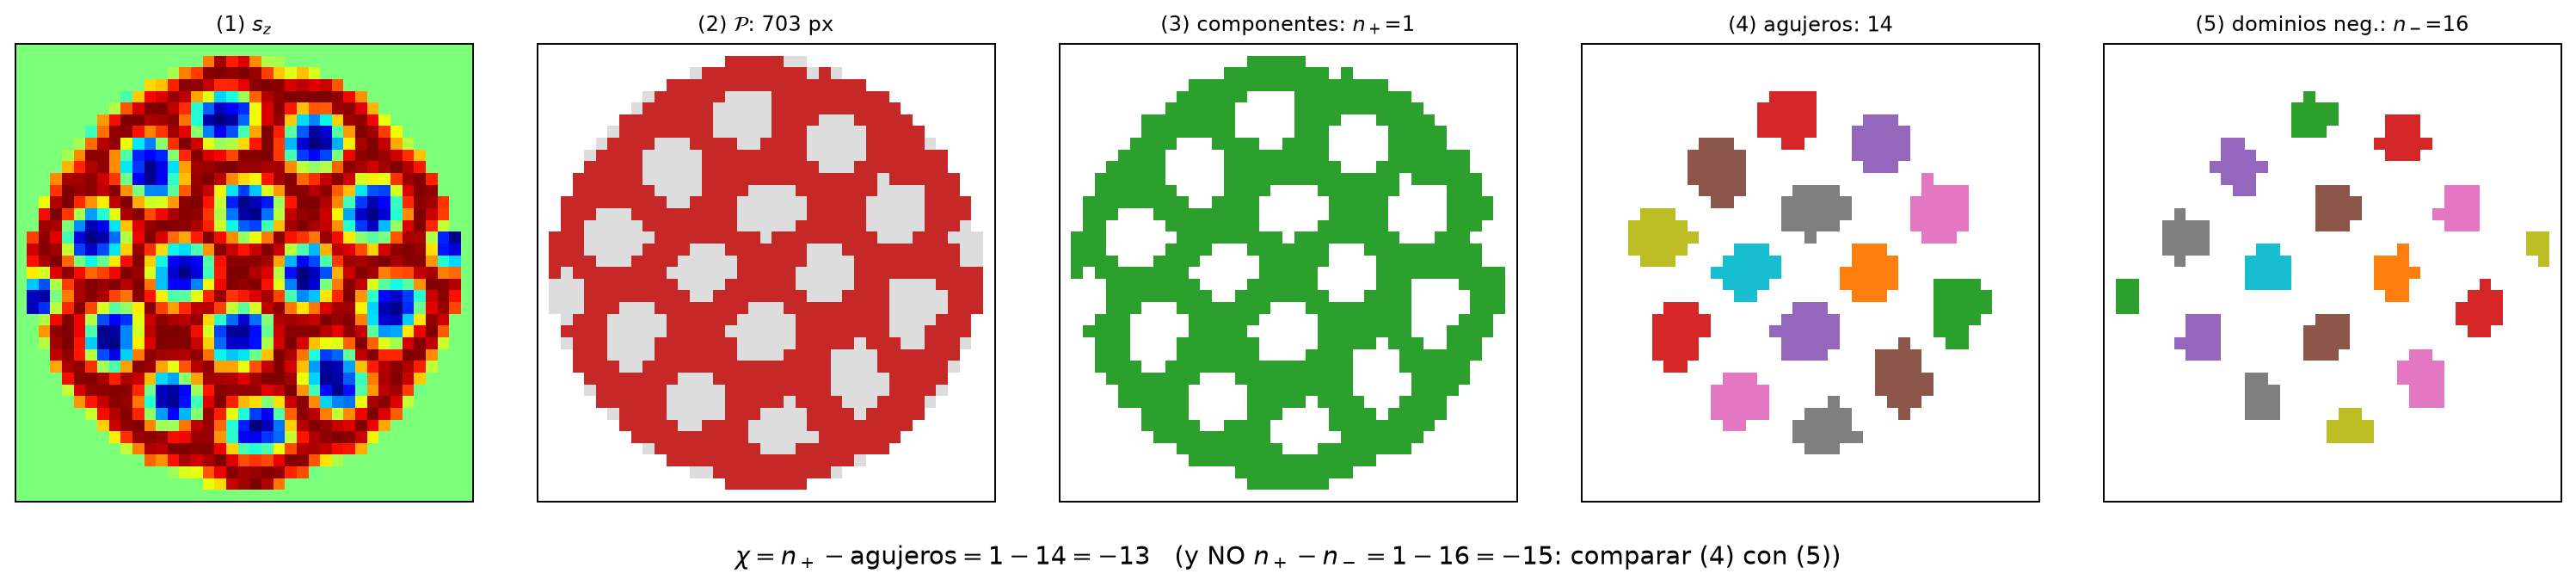
\includegraphics[width=\textwidth]{topo_steps.png}
  \caption{The same computation on one configuration of cluster 16 (Skyrmions). Panel (2)
  thresholds at $+0.25$; panel (3) finds the components of $\mathcal{P}$, here a single
  connected background; panel (4) shows the enclosed pieces of the complement, which can be
  counted one by one. Panel (5) is the negative set, shown to make the difference visible:
  it has $16$ domains while $\mathcal{P}$ has $14$ holes, because domains joined through
  the intermediate band $|s_z|\le0.25$ merge into one hole, and a domain reaching the disk
  edge encloses nothing.}
\end{figure}

Reading the numbers off the figure:
\[
  n_+ = 1, \qquad \text{holes} = 14, \qquad
  \chi = 1 - 14 = \mathbf{-13},
\]
and the descriptor returns exactly $-13$. Note what $\chi$ is \emph{not}: with $n_-=16$,
the quantity $n_+ - n_- = 1-16 = -15$, a different number. The eye counts bubbles in panel
(5); $\chi$ counts holes in panel (4).

The five descriptors of this one image:
\begin{center}\small
\begin{tabular}{lrl}
\toprule
$n_+$ & 1 & one connected positive background \\
$n_-$ & 16 & sixteen negative domains \\
$\chi$ & $-13$ & $1$ component minus $14$ holes \\
$w$ & 0.142 & $14.2\%$ of neighbour pairs cross a wall \\
$a_{\max}$ & 0.670 & the background covers $67\%$ of the disk \\
\bottomrule
\end{tabular}
\end{center}

\subsection{From one image to a table}

Each of those five numbers is computed on \emph{one} configuration. The table in
Section~5 summarises $1{,}500$ configurations per cluster, and each column is the median of
its own list. For cluster 16 the individual $\chi$ values begin
$-4,\,-4,\,-10,\,-10,\,-10,\,-8,\,-14,\,-9,\,-21,\,-6,\dots$ and the table reports their
median, $-10$. Columns therefore cannot be combined arithmetically: the median of $n_+$
minus the median of $n_-$ is not the median of $\chi$, nor of anything else.

\section{How it is computed}

\begin{enumerate}
  \item Threshold inside the disk to obtain the binary sets $\mathcal{P}$ and $\mathcal{N}$.
  \item Label connected components with \textbf{8-connectivity}
        (\texttt{scipy.ndimage.label}). Eight rather than four because two domains touching
        only at a corner are physically one domain.
  \item $\chi$ from \texttt{skimage.measure.euler\_number} on $\mathcal{P}$.
  \item $w$: sweep horizontal and vertical neighbour pairs inside the disk and count those
        with $s_z(i)\,s_z(j)<0$ --- a sign change between adjacent cells is a domain wall
        crossing --- normalised by the number of valid pairs.
  \item $a_{\max}$: largest component area divided by the disk area.
\end{enumerate}

Cost is $0.33$\,ms per image, so the full dataset of $169{,}671$ configurations takes under
a minute on one core. Implementation: \texttt{notebooks/utils/\allowbreak metrics.py},
\texttt{topological\_descriptors} and \texttt{topological\_batch}.

\section{Examples}

\begin{figure}[H]
  \centering
  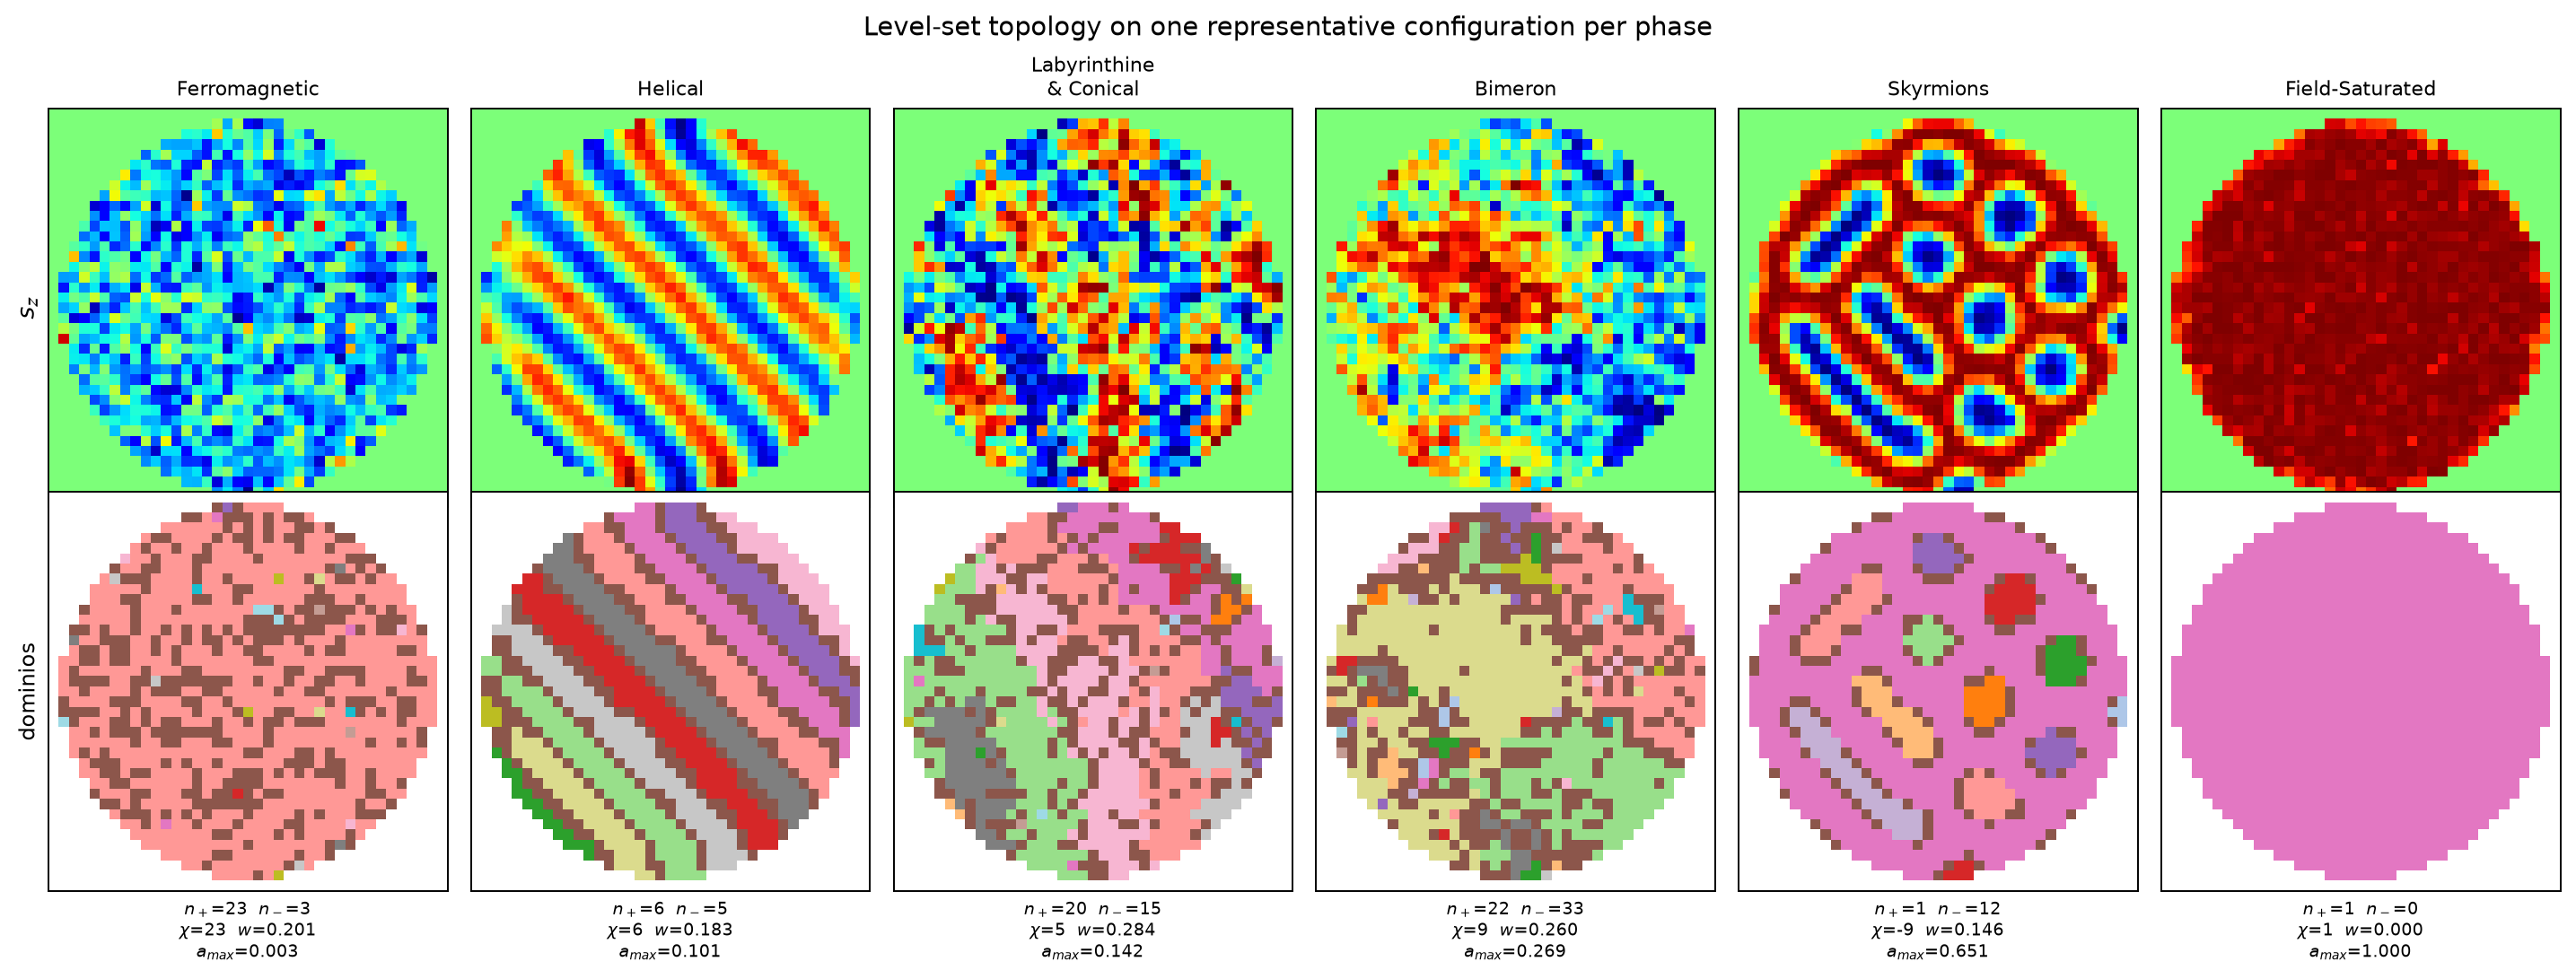
\includegraphics[width=\textwidth]{topo_phases.png}
  \caption{One representative configuration per phase, chosen as the sample closest to its
  phase's median $\chi$. Top: $s_z$ with the scale pinned to $[-1,1]$. Bottom: the labelled
  domains, one colour per connected component. The sign of $\chi$ separates the families:
  $\chi=-9$ for Skyrmions, where isolated bubbles perforate the background, against
  $\chi=+6$ for Helical stripes and $\chi=+1$ for the saturated state, a single domain
  filling the disk ($a_{\max}=1.000$).}
\end{figure}

\begin{figure}[H]
  \centering
  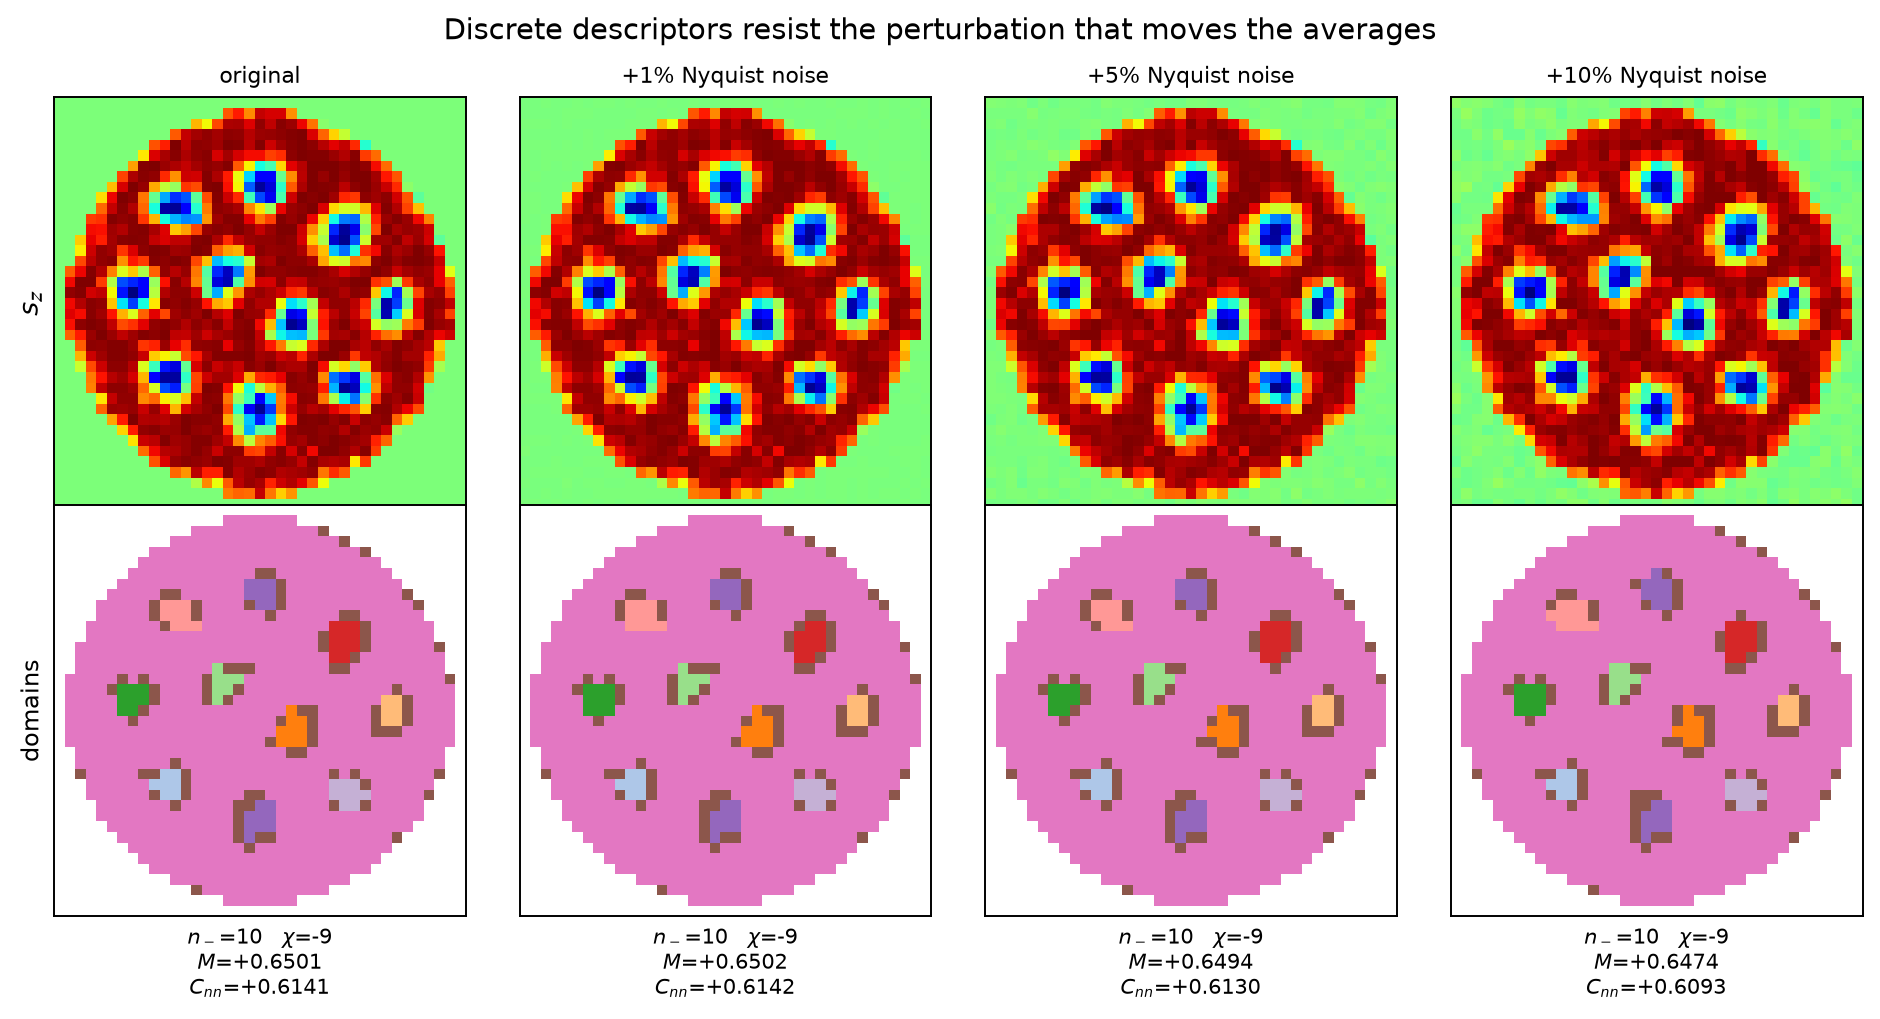
\includegraphics[width=0.86\textwidth]{topo_robust.png}
  \caption{The property that motivates the descriptor. Noise is added at the Nyquist
  frequency --- the band where latent guidance writes --- at $1\%$, $5\%$ and $10\%$ of the
  image range. $\chi$ is unchanged throughout and the domain count is unchanged up to $5\%$;
  at $10\%$ one extra domain appears, $n_-$ going from 12 to 13. To move a count at all one
  has to merge, destroy or create a domain, which is a structural change rather than a
  change of amplitude, and it takes ten times the perturbation that latent guidance uses.}
\end{figure}

\section{Results}

\subsection{Descriptor values by phase}

Medians over a stratified sample of $16{,}850$ configurations ($1{,}500$ per cluster id
where available); $w$ and $a_{\max}$ are means.

\begin{table}[H]
\centering\small
\begin{tabular}{llrrrrr}
\toprule
Phase & id & $n_+$ & $n_-$ & $\chi$ & $w$ & $a_{\max}$ \\
\midrule
\multirow{3}{*}{Ferromagnetic}
                       & 10 & \warn{36} & \warn{37} & \warn{$+36$} & \warn{0.372} & \warn{0.005} \\
                       & 11 & 29 & 13 & $+16$ & 0.229 & 0.352 \\
                       & 12 & 0  & 1  & $0$   & 0.008 & 0.000 \\
\midrule
\multirow{3}{*}{Helical}
                       & 4  & 11 & 11 & $+7$ & 0.221 & 0.117 \\
                       & 5  & 9  & 9  & $+6$ & 0.219 & 0.111 \\
                       & 13 & 5  & 7  & $+4$ & 0.188 & 0.206 \\
\midrule
\multirow{2}{*}{Labyrinthine \& Conical}
                       & 6  & 17 & 18 & $+6$ & 0.217 & 0.188 \\
                       & 14 & 2  & 7  & $+1$ & 0.118 & 0.335 \\
\midrule
Bimeron                & 8  & 22 & 22 & $+8$ & 0.243 & 0.250 \\
\midrule
\multirow{2}{*}{Skyrmions}
                       & 15 & 1 & 10 & \best{$-4$}  & 0.114 & 0.748 \\
                       & 16 & 1 & 12 & \best{$-10$} & 0.106 & 0.767 \\
\midrule
Field-Saturated        & 17 & 1 & 0  & $+1$ & 0.000 & \best{1.000} \\
\bottomrule
\end{tabular}
\end{table}

Skyrmions are the only family with $\chi<0$, and Field-Saturated the only one with
$a_{\max}=1$. Both fall out of the descriptor without any tuning.

\paragraph{An observation on the Ferromagnetic grouping.}
The three cluster ids merged into \emph{Ferromagnetic} are topologically very different.
Id 12 is a single domain covering the disk with the opposite sign to id 17 --- the mirror of
the saturated state, and ferromagnetic in the ordinary sense. Id 10 fragments into
36 domains whose largest covers $0.5\%$ of the disk, with $37\%$ of neighbour pairs
straddling a wall: that is a disordered configuration, not an ordered one. Id 10 holds
$15{,}584$ samples, so this is not a marginal case. Whether the grouping is deliberate is a
question for the physics, but the numbers should be on record.

\subsection{Agreement with the existing phase labels}

A random forest on five descriptors, five-fold cross-validated, on a sample drawn with the
dataset's natural class proportions (Helical $59.5\%$, Ferromagnetic $15.0\%$,
Labyrinthine $11.9\%$, Skyrmions $6.3\%$, Field-Saturated $3.6\%$, Bimeron $3.6\%$).
Given that imbalance, balanced accuracy is the honest column: always predicting Helical
already scores $0.595$ on plain accuracy.

\begin{table}[H]
\centering
\begin{tabular}{lccc}
\toprule
Features & Accuracy & \best{Balanced accuracy} & Macro F1 \\
\midrule
always predict Helical      & 0.595 & --- & --- \\
three physical scalars      & 0.890 & 0.813 & 0.821 \\
\best{five topological}     & 0.901 & \best{0.831} & 0.837 \\
\best{both families}        & \best{0.934} & \best{0.888} & \best{0.897} \\
\bottomrule
\end{tabular}
\end{table}

Topology alone edges out the three scalars, and the union gains $7.5$ points of balanced
accuracy over the scalars alone. The descriptors carry information the averages do not.

\begin{table}[H]
\centering\small
\caption{Per-phase recall with both families combined.}
\begin{tabular}{lcr}
\toprule
Phase & Recall & $n$ \\
\midrule
Field-Saturated         & 99.9\% & 728 \\
Ferromagnetic           & 99.5\% & 3002 \\
Skyrmions               & 98.1\% & 1267 \\
Helical                 & 96.8\% & 11904 \\
Labyrinthine \& Conical & \warn{71.9\%} & 2378 \\
Bimeron                 & \warn{66.4\%} & 721 \\
\bottomrule
\end{tabular}
\end{table}

The two weak classes are confused with each other and with Helical, which is physically
reasonable: a labyrinth is disordered stripes and a bimeron sits between the two. The
classifier reaching $99.5\%$ on Ferromagnetic does not resolve the grouping question above
--- with enough data it simply learns all three modes.

\section{Why this matters for the generative models}

Every physical figure of merit reported so far answers ``do the averages agree''. These
descriptors answer a stricter question: \emph{did the model produce the phase it was asked
for}. That distinction is what the robustness figure is about. A generator whose
magnetisation, correlation and peak wavevector all match the reference while its domain
counts do not is reproducing the statistics with the wrong structures, and only a discrete
descriptor will say so.

It also gives a cheap phase classifier --- $0.33$\,ms per image, five interpretable numbers,
$0.888$ balanced accuracy, no neural network --- which can be applied to generated samples
directly.

\end{document}
